\chapter{Introduction}\label{ch:intro}

\section{Searching for Exoplanets}\label{sec:ch1_background}
The idea that there could be planets orbiting stars other than our own sun has been around for at least four hundred years, with historical proponents ranging from Giordano Bruno to Isaac Newton.  It was not until 1988, however, that the first confirmed discovery of an extra-solar planet (or exoplanet) was made \citet{campbell1988search}, and not until 1995 that a planet was discovered about a star similar to the sun \citet{mayor1995jupiter}.  In the fifteen years since then, new planets have been discovered at an ever accelerating rate, as evidenced by \reffig{fig:planDiscHist}.
\begin{figure}[ht]
 \center
 \includegraphics[width=5.5in]{./figures/planDiscHist}
  \caption[History of exoplanet discovery]{ \label{fig:planDiscHist} Number of confirmed exoplanets as a function of year.  There are currently 531 known exoplanets, and over 1200 planetary candidates.  Data retrieved from the NASA/IPAC/NExScI Star and Exoplanet Database \url{http://nsted.ipac.caltech.edu} on April 17th, 2011.}
\end{figure} 

Our ability to find large numbers of exoplanets is the key to our eventual understanding of planet formation and evolution.  To understand why, we need only look at the history of astrophysics and our knowledge of the formation and evolution of stars and galaxies.  Stellar and galactic evolution take place on time scales so vast that not even multiple generations of astronomers could hope to see many changes in the stars in our sky.  However, despite having only a static view of these dynamic processes, we are lucky enough to have an incredibly large sample of observable objects, all at various stages of development.  This large data set, along with the convenient fact that looking further into the universe is equivalent to looking further back in time, has allowed us to deduce the processes by which stars are formed, evolve, and eventually transform into a variety of other interesting objects.  We've gained confidence in these models based on our ability to locate stars at each stage of the process.  With a sufficiently large pool of observed exoplanets, we can expect the same outcome for planet science.

Unfortunately, observing exoplanets is significantly harder than observing stars.  There are no examples of bright exoplanets that can be seen with the naked eye or simple instrumentation, and so we must find each exoplanet before studying it.  In many ways, this searching for exoplanets is closer to particle physics than to traditional observational astronomy.  In each case, we search for something that may not be there, guided only by constantly evolving theory.  Similarly, both new planets and new particles are often detected indirectly, based on their effects on more easily observed objects.  Finally, both pursuits require complex dedicated equipment, which often represents the extreme borders of current technology and large investments of resources.  To answer these challenges, the exoplanet community has developed new instrumentation and data analysis methods and even whole new methods for detecting the presence of exoplanets, leading to the accelerating rate of discoveries described above. 

Alongside the various planet-finding surveys, there has been a concurrent effort to develop detailed models and simulations of observatory operations and planet observations.  These simulations serve three main purposes:  first, they allow the community to directly compare the expected scientific returns of proposed observatory and mission concepts.  Second, they can be used to optimize target selection and observation scheduling for existing facilities, while providing a controlled testing environment for data processing pipelines.  Finally, the ability to calculate the probability that a planet of a given type will be observed with a given frequency, conditional on a planet formation model, means that observations can be used to choose between competing planet evolution theories and closely estimate absolute planet frequencies. 

These applications have already been proven to be helpful in both the mission planning and the data analysis.  For example, the Kepler Mission, which has more than doubled the number of exoplanet candidates since its launch in 2009, utilizes the Kepler end-to-end model---an integrated simulation used to  test the data processing pipeline and simulate observatory operations \citep{bryson2010kepler}.  Similarly, there have been many statistical analyses of the existing exoplanet data set that relied heavily on observation modeling, including the analysis of 
radial velocity surveys in \citet{cumming2008} and a microlensing study described in \citet{gould2010frequency}.

This thesis will explore exoplanet observation modeling in relation to all of these applications.  We will start by formulating a standardized set of parameters for use throughout the rest of the chapters.  The remainder of this chapter will introduce the variables required to describe how planets orbit their parent (or host) stars and how their position and motion in space can be defined with respect to a specific observer.  We will also detail how light from stars and planets interacts with imaging systems to produce the images that form the raw data for many planet-finding methods.  

This description will be continued in \refch{ch:obs_methods} with a detailed discussion of four methods used to study exoplanets.  These are: doppler spectroscopy, which produced the majority of exoplanet detections before 2010, precision astrometry, which has the potential of allowing us to detect planets much smaller than those currently being found, transit photometry, which, thanks to the Kepler mission, has more than doubled the number of exoplanet candidates, and finally direct detection, which promises to become a very powerful tool in the near future, and has already produced a number of fascinating discoveries.  The first three of these methods, doppler spectroscopy, astrometry, and transit photometry, are indirect---they rely on observations of the star in order to infer the presence of planets, tracking the star's motion in the case of astrometry and doppler spectroscopy, and the amount of light coming from the target system in the case of transit photometry.  Direct detection is the only method that attempts to image the exoplanets themselves.  Each of these methods has specific strengths and limitations, all of which will be discussed in detail.

\refch{ch:param_dists} will review what we currently know about exoplanets, and introduce the idea of a statistical approach to exoplanet study, focusing on properties of populations of planets rather than specific examples.  Based on the formalism laid out in the first two chapters, we will develop a statistical description of planetary orbits, which will be applied to the optimization of planet-finding surveys.  In the course of this discussion we will introduce the concept of completeness, which allows for a systematic way of incorporating instrument biases into the analysis of generated data.

\refch{ch:obs_sims} will discuss the various components required to build complete simulations of exoplanet observations.  Starting with the generation of sample exoplanetary systems, we will track each step of how a realistic data set can be generated for each observation method.  We will also explore how to propagate systems forward in time so that we can simulate entire surveys in addition to individual observations.  These techniques will be applied to the construction of an integrated simulation capability for direct detection planet-finders, which will be employed in a series of case studies to explore the performance of multiple proposed missions.

Finally, \refch{ch:int_data} will consider the data analysis problem, and will demonstrate how the formalism built up throughout the thesis, along with the well-developed field of optimal estimation, can be used to systematically generate complex planetary system models from multiple varied data streams.  Taking into account the accelerating rate of discovery and the proliferation of observation methods, it is highly likely that these are the kinds of data sets the exoplanet community will have at its disposal in the near future, and the applications described in this chapter are a first step towards taking advantage of the increased information that can be extracted thanks to detailed modeling and simulation.

\section{Exosystem Parameters}\label{sec:exosystem_params}

Before proceeding, it is important to define a consistent description of all of the physical quantities that will be treated in later chapters.  This section defines every variable that will be used in multiple contexts so as to preserve a uniform notation throughout.

\begin{figure}[ht] 
 \center
 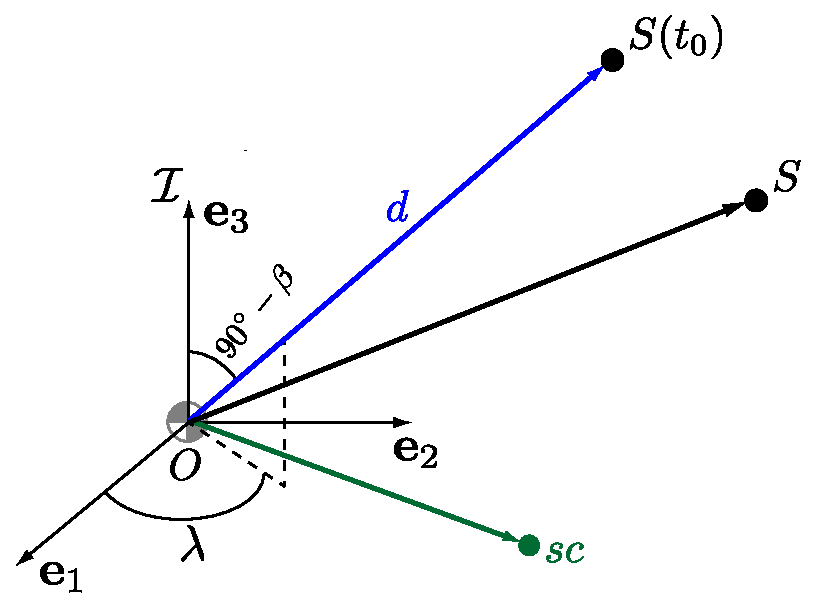
\includegraphics[width=4.5in]{./figures/barycentric_frame}
  \caption[Inertial barycentric/ecliptic frame]{ \label{fig:baryFrame} The inertial barycentric/ecliptic frame $\mc I$ with origin $O$ at the solar system barycenter.  Star $S$ is at coordinates $\lambda, \beta$ and distance $d$ at reference epoch $t_0$.}
\end{figure} 
The position of an exosystem primary star (or `target' star) is denoted by $S\addsymbol{$S$}{Star position}$, and, when expressed with respect to some specific point $P$, is given by the vector $\R_{S/P}$.  The observer location is denoted by point $sc\addsymbol{$sc$}{Observer position}$, which may represent a space or ground-based observatory.  We sometimes find it useful to define the star position via a celestial coordinate system.  Typically, we use a barycentric/ecliptic frame $\mc I = (O, \mf e_1,\mf e_2, \mf e_3)\addsymbol{$\mc I$}{Inertial barycentric/ecliptic solar system frame.}$ whose origin $O\addsymbol{$O$}{Solar system barycenter}$ is at the solar system barycenter (see \reffig{fig:baryFrame}).   In this frame, coordinates $(\lambda,\beta)$ along with the target star distance $d\addsymbol{$d$}{Star distance with respect to solar system barycenter}$ define the star position as:
\begin{equation}
\left[\R_{S/O}\right]_\mathcal{I}  =  d\left[ \begin{array}{c} \cos \lambda \cos \beta \\ \sin \lambda \cos \beta \\ \sin \beta \end{array}\right] \,,
\end{equation}
where
\begin{equation}
d \triangleq \Vert \mf r_{S/O} \Vert \,.
\end{equation}
It is important to note that $(\lambda$, $\beta)$ and $d$ are typically catalogued values, and thus define the star position at a specific epoch ($t_0$), whereas the star-pointing vector with respect to the solar system barycenter and the observer is constantly changing.

Similarly, the position of a planet is given by point $P\addsymbol{$P$}{Planet position}$ and the exosystem barycenter is defined as $G\addsymbol{$G$}{Exosystem barycenter}$.  In cases with multiple planets in one exosystem, the planet positions are enumerated as $P_i$. The star-planet separation vector is given by:
\begin{equation}
\R_{P/S} \triangleq \R_{P/G} - \R_{S/G} \,.
\end{equation}
The time varying orbital radius, $r\addsymbol{$r$}{Orbital radius}$ is equal to the magnitude of the star-planet vector:
\begin{equation}
r  \triangleq  \Vert \R_{P/S} \Vert \,.
\end{equation}
The planet's geometric albedo and radius are given by $p\addsymbol{$p$}{Geometric albedo}$  and $R\addsymbol{$R$}{Planet radius}$, respectively, and the total flux of the planet and star are given by $F_p\addsymbol{$F_p$}{Planet flux}$  and $F_s\addsymbol{$F_s$}{Star flux}$, respectively.  The intrinsic luminosity of the star is given by $L\addsymbol{$L$}{Stellar luminosity}$ measured in $L_\odot$ (solar luminosity).

It is frequently useful to describe planetary orbits via Keplerian orbital elements.  These are derived from the solution of the two-body problem, and are an exact description of planetary motion in the case of a single-planet exosystem.  In systems with multiple planets, the orbits may still be approximated as Keplerian, although this ignores all planet-planet interactions and therefore cannot exactly predict future positions of all of the system bodies.  This can still be a useful approximation, however, as no analytic solution exists to the general n-body problem.  As we will see, there are actually two different ways of approximating n-body systems via Keplerian orbital elements: we can either fit an average ellipse to multiple orbits worth of data, producing an average set of Keplerian elements, or we can calculate time-varying Keplerian elements to reflect the perturbations due to the other bodies in the system.  In the latter case, we typically use osculating Keplerian elements---i.e., the orbital elements of the Keplerian orbit tangent to the true orbit at that point in time.

The difference between constant, osculating, and averaged Keplerian orbital elements is very important as they describe very different things.  With a fixed Keplerian orbit, you can predict the position and velocity of the planet for all time.  If there are no perturbations on the planet, this position and velocity will be correct.  With perturbations, however, the true position and velocity will progressively deviate from the ones predicted by the Keplerian orbit.  An averaged set of orbital elements will never exactly match the planet's true position and velocity, but will minimize the position error over an entire data set.  Osculating orbital elements will always give you the correct position and velocity, but require knowledge of the perturbations acting on the planet.

Furthermore, while a constant set of Keplerian elements describes a particular ellipse corresponding to the planet's orbit, osculating elements are much more difficult to interpret, as they only correspond to the instantaneously tangential orbit.  This means that in certain cases the osculating orbit will be highly eccentric while the planet's orbit is actually nearly circular\footnote{This is particularly true for resonant orbits \citep{tinney20062}.}.  Throughout this thesis, we will employ both types of orbital elements.  When dealing with single planet system simulations, as in \S\ref{sec:sysProp}, we will employ constant Keplerian orbital elements.  When using orbital elements to talk about multi-planet systems, as we do later in this section, we will use osculating orbital elements.  Finally, when discussing how certain detection methods that rely on finding periodic signals to detect planets, we will employ averaged orbital elements (see \refch{ch:obs_methods} and \S\ref{sec:state_init_apri}).

\begin{figure}[ht]
 \center
 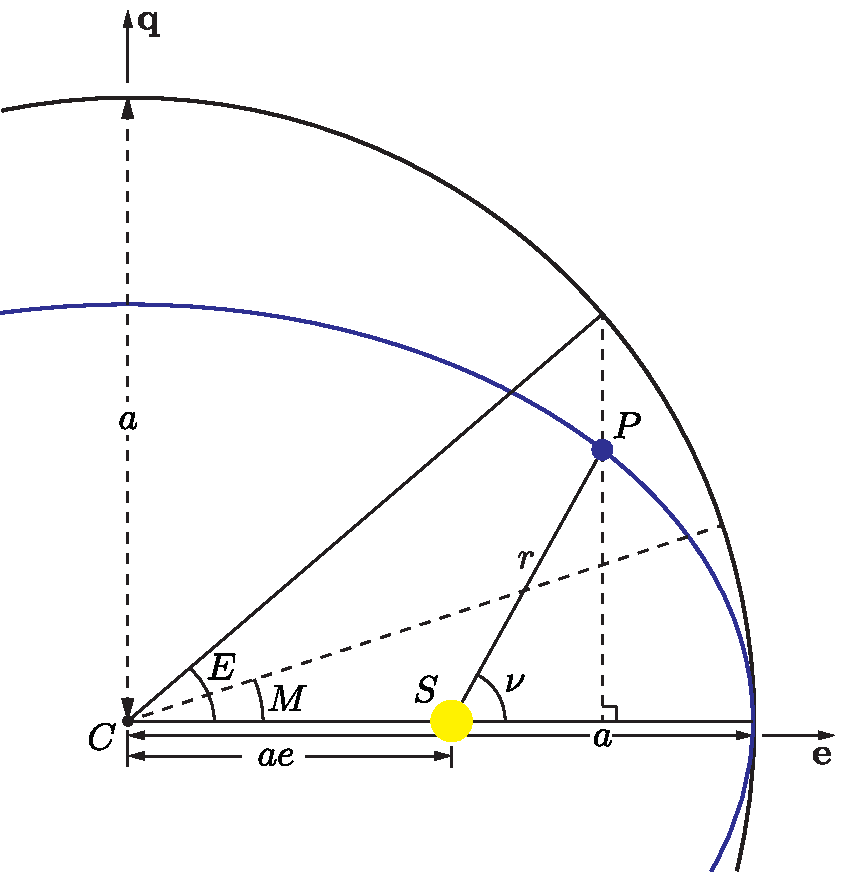
\includegraphics[width=4.5in]{./figures/anomaly_diagram}
  \caption[Anomaly Diagram]{ \label{fig:anomaly_diagram} Schematic of a Keplerian orbit (blue ellipse) and auxiliary circle (black ellipse).  The auxiliary circle has a radius equal to the orbit's semi-major axis, with center $C$.}
\end{figure} 
We define a Keplerian orbit via the parameter set $(a,e,\psi,\theta,\phi)$ where $a\addsymbol{$a$}{Orbital semi-major axis}$ is the semi-major axis, $e\addsymbol{$e$}{Orbital eccentricity}$ is the eccentricity, and $\psi,\theta,\phi\addsymbol{$\psi,\theta,\phi$}{Euler angles orienting orbit in space}$ are Euler angles determining the orientation of the orbit in the observer's reference frame\footnote{Of course, there exist many other ways of orienting the planar orbit in three dimensions.  For further discussions on some alternatives to the Euler angles, see \S\ref{sec:state_selection}.}.  The position of the planet on its orbit at the time of observation is given by either the mean anomaly $M\addsymbol{$M$}{Mean anomaly}$, eccentric anomaly $E\addsymbol{$E$}{Eccentric anomaly}$, or the true anomaly $\nu\addsymbol{$\nu$}{True anomaly}$. In a 2-body system, the planet's orbit lies in a single plane, and thus can be fully described using only scalar values, as shown in \reffig{fig:anomaly_diagram}.  Keplerian orbits are conic sections---closed planetary orbits are ellipses with the star located at one focus.  The orbital radius is defined in terms of the eccentricity, semi-major axis, and true anomaly as:
\begin{equation} \label{eq:rdef}
r = \frac{a(1-e^2)}{e \cos(\nu) + 1} \,.
\end{equation}

The orbital velocity and radius vary as functions of the true anomaly, which is defined as the angle between the current star-planet vector and the star-planet vector at the time of periapsis passage (see \reffig{fig:anomaly_diagram}).  Using the planar orbital representation, we can write the planet position and velocity  with respect to the star as:
\begin{align} 
\mf r_{P/S} &= r\left(\cos\nu \hat{\mf e} + \sin\nu \hat{\mf q}\right) \label{eq:planPosVect}\\
{}^\mc I \mf v_{P/S} &= \fddt{I} \mf  r_{P/S} = \sqrt{\frac{\mu_P + \mu_S}{\ell}}\left(-\sin\nu \hat{\mf e} + (e + \cos\nu) \hat{\mf q}\right)\label{eq:planVelVect}
\end{align}
where $\mu_P\addsymbol{$\mu_P$}{Gravitational parameter of planet}$ and $\mu_S\addsymbol{$\mu_S$}{Gravitational parameter of star}$ are the gravitational parameters of the star and planet, respectively, equal to the product of their masses ($m_S\addsymbol{$m_S$}{Mass of star}$ and $m_P\addsymbol{$m_P$}{Mass of planet}$) and the universal gravitational constant $G$.  The semi-latus rectum of the ellipse, $\ell$, is given geometrically as:
\begin{equation}\label{eq:semilatusrectum}
\ell = a(1 - e^2) \,.
\end{equation}
The unit vector $\hat{\mf e}$ (known as the normalized eccentricity vector) can be expressed as:
\begin{equation}\label{eq:eccenVec}
\hat{\mf e} = \left<\frac{1}{\mu_S + \mu_P}\left[\left( \Vert{}^\mc I \mf v_{P/S}\Vert^2 - \frac{\mu_S + \mu_P}{r}\right) \mf r_{P/S} - \left( \mf r_{P/S} \cdot {}^\mc I \mf v_{P/S}\right){}^\mc I \mf v_{P/S}\right]\right> \,.
\end{equation}
The orthogonal unit vector $\hat{\mf q}$ can be written as:
\begin{equation}\label{eq:qvecdef}
\hat{\mf q} = \left<\mf r_{P/S} \times {}^\mc I \mf v_{P/S}\right> \times \hat{\mf e}\,.
\end{equation}
These two unit vectors, $\hat{\mf e}$ and $\hat{\mf q}$, define the perifocal reference frame.  From \refeq{eq:qvecdef} we can see that the third vector of this frame, $\hat{\mf h} = \hat{\mf e} \times \hat{\mf q}$, is the direction of the orbit's normalized angular momentum:
\begin{equation} \label{eq:angMomentum}
{}^\mc I \mf h_{P/S} =  \mf r_{P/S} \times {}^\mc I \mf v_{P/S} \,,
\end{equation}
which is always orthogonal to the plane of the orbit.

To aid in calculating the planet position, it is useful to define an auxiliary circle with a radius equal to the orbit's semi-major axis and centered at the orbit's  center.  This allows us to define a mean anomaly, a central angle describing the mean planetary motion, given by:
\begin{equation} \label{eq:Mdef}
M \triangleq 2\pi \frac{t-t_p}{P_{orb}} \,,
\end{equation}
where $P_{orb}\addsymbol{$P_{orb}$}{Orbital period}$ is the orbital period, $t\addsymbol{$t$}{Time}$ is the current time, and $t_p$ is the time of the last periapsis passage (closest planet approach to the star).  The orbital period is:
\begin{equation}\label{eq:Pdef}
P_{orb} = 2\pi\sqrt{\frac{a^3}{\mu_S +\mu_P}} \,.
\end{equation}
The mean anomaly is proportional to the area covered by $\mf r_{P/S}$ since periapsis passage, and is thus linear in time.  The eccentric anomaly is related to the mean anomaly via the Kepler equation:
\begin{equation} \label{eq:EtoM}
M = E - e\sin(E) \,,
\end{equation}
and related to the true anomaly as:
\begin{equation} \label{eq:nutoE}
\tan\left(\frac{\nu}{2}\right) =\sqrt{\frac{1+e}{1-e}} \tan\left(\frac{E}{2}\right) \,.
\end{equation}

To orient the orbit in some observer's reference frame $\mc A$, we apply a 3-1-3 rotation using the angle set $(\psi,\theta,\phi)_{\mc A}$ \citep{kane}:
\begin{equation}\label{eq:rpsrot}
[\mf r_{P/S}]_{\mc A}  =
\left[ \begin{matrix} \cos\phi &\sin\phi & 0 \\ -\sin\phi& \cos\phi & 0 \\ 0 & 0 & 1 \end{matrix}\right]
\left[ \begin{matrix} 1 & 0 & 0 \\ 0 & \cos\theta &\sin\theta \\0 & -\sin\theta & \cos\theta \end{matrix}\right]
\left[ \begin{matrix} \cos\psi &\sin\psi & 0 \\ -\sin\psi & \cos\psi & 0 \\ 0 & 0 & 1 \end{matrix}\right]
[\mf r_{P/S}]_{\mc P}   \,,
\end{equation}
where $\mc P$ is a reference frame whose first two unit vectors lie in the $\hat{\mf e},  \hat{\mf q}$ plane and whose third unit vector is in the $\hat{\mf h}$ direction
(see \S\ref{sec:direct_detection} for an example of one such frame).  The  $\mc P$ frame is inertial only in the case of a non-accelerating frame origin, which results in another difficulty in using the Keplerian description as this makes $\mc P$ a heliocentric frame.  Note that we have used left-handed rotations here to conform to conventions in the literature (cf.~\citet{vinti}).  We can use these rotations to convert between the Keplerian orbital elements and the heliocentric planet position and velocity, simply by by expressing the planar orbit as:
\begin{equation}\label{eq:rpsP1}
[\mf r_{P/S}]_{\mc P}  = \left[\begin{matrix} r \cos \nu \\ r \sin \nu \\ 0 \end{matrix} \right] = \left[\begin{matrix} a (\cos E - e) \\ b \sin E \\ 0 \end{matrix} \right] \,,
\end{equation}
where $b$ is the semi-minor axis of the orbit, given by:
\begin{equation}
b = a\sqrt{1 - e} \,,
\end{equation}
and we take the angle set $(\psi,\theta,\phi) = (\Omega, I, \omega)$ where $\Omega\addsymbol{$\Omega$}{Longitude of the ascending node}$ is the longitude of the ascending node, $I\addsymbol{$I$}{Inclination}$ is the inclination and $\omega\addsymbol{$\omega$}{Argument of periapsis}$ is the argument of periapsis.  The velocity vector is found by differentiating the position, yielding:
\begin{equation}\label{eq:vpsP1}
[{}^\mc P \mf v_{P/S}]_{\mc P} = \fddt{P}{[\mf r_{P/S}]_{\mc P}} =  \sqrt{\frac{\mu_S + \mu_P}{a}}\frac{1}{1 - e\cos E} \left[\begin{matrix} -\sin E\\ \sqrt{1 - e}\cos E \\ 0 \end{matrix} \right] \,.
\end{equation}
 There are multiple algorithms for converting heliocentric position and velocity vectors to Keplerian orbital elements.  One of the most straight-forward, described in \citet{vinti}, assumes a planar orientation as in \refeq{eq:rpsrot} and then calculates the semi-major axis and semi-latus rectum from the orbital energy and angular momentum:
\begin{align}
a = -\frac{\mu_S + \mu_P}{2E} &= -\frac{\mu_S + \mu_P}{2}\left[ \frac{\Vert {}^\mc I \mf v_{P/S} \Vert^2}{2} -\frac{\mu_S + \mu_P}{\Vert \mf r_{P/S}\Vert}\right]^{-1} \,, \label{eq:vec2orbelem1} \\
\ell &= \frac{{}^\mc I \mf h_{P/S}}{\mu_S + \mu_P} \frac{\Vert  \mf r_{P/S} \times  {}^\mc I \mf v_{P/S} \Vert}{\mu_S + \mu_P} \,.
\end{align}
The eccentricity can then be calculated via \refeq{eq:semilatusrectum}:
\begin{equation}
e = \sqrt{1 - \frac{\ell}{a}} \,.
\end{equation}
Given inertial frame unit vectors $(\mf e_1, \mf e_2, \mf e_3)$, we can write:
\begin{align}
\cos I &= \frac{(\mf r_{P/S} \times  {}^\mc I \mf v_{P/S}) \cdot \mf e_3}{\Vert \mf r_{P/S} \times  {}^\mc I \mf v_{P/S}\Vert} \label{eq:cosI}\,,
\\
\sin I  &= \frac{\Vert  \mf e_3 \times (\mf r_{P/S} \times  {}^\mc I \mf v_{P/S}) \Vert}{\Vert \mf r_{P/S} \times  {}^\mc I \mf v_{P/S}\Vert} \,,
\\
\cos \Omega &= -\frac{(\mf r_{P/S} \times  {}^\mc I \mf v_{P/S}) \cdot \mf e_2}{\Vert \mf r_{P/S} \times  {}^\mc I \mf v_{P/S}\Vert \sin I} \,,
\\
\sin \Omega  &= \frac{(\mf r_{P/S} \times  {}^\mc I \mf v_{P/S}) \cdot  \mf e_1}{\Vert \mf r_{P/S} \times  {}^\mc I \mf v_{P/S}\Vert \sin I} \,,
\\
\cos \omega &= \frac{1}{e\sin I} \left(\frac{\Vert \mf r_{P/S} \times  {}^\mc I \mf v_{P/S} \Vert \left( {}^\mc I \mf v_{P/S} \cdot \mf e_3\right)}{\mu_S + \mu_P} - \frac{ \Vert \mf r_{P/S} \times  {}^\mc I \mf v_{P/S} \times \mf r_{P/S}  \Vert}{\Vert \mf r_{P/S} \times  {}^\mc I \mf v_{P/S} \Vert \Vert \mf r_{P/S} \Vert}\right) \,,
\\
\sin \omega  &= \frac{1}{e\sin I} \left(\frac{ \Vert  {}^\mc I \mf v_{P/S} \times \mf r_{P/S} \times  {}^\mc I \mf v_{P/S} \Vert}{\mu_S + \mu_P} - \frac{ \mf r_{P/S} \cdot \mf e_3}{\Vert \mf r_{P/S} \Vert}  \right) \label{eq:sinO}\, .
\end{align}
With both sine and cosine expressions for an angle, the angle may be reconstructed over the full range of $[0, 2\pi]$ with the two argument arctangent function:
\begin{equation}
\textrm{atan2}(y,x) = \left\{\begin{array}{l l}
\tan^{-1}\left(y/x\right) & x > 0\\
\pi + \tan^{-1}\left(y/x\right) & x < 0, y \ge 0\\
-\pi + \tan^{-1}\left(y/x\right) & x < 0, y < 0\\
\pi/2 & x =  0, y > 0\\
-\pi/2 & x = 0, y < 0
\end{array} \right.
\end{equation}
where $y = \cos\theta$ and $x = \sin\theta$.  Thus Equations (\ref{eq:cosI}) through (\ref{eq:sinO}) can be used to precisely orient the orbit in the unit sphere given a single measurement of the position and velocity vectors.  The time varying Keplerian orbital element (anomaly) can similarly be found by using:
\begin{align}
\cos E &= \frac{1}{e}\left(1 - \frac{\Vert \mf r_{P/S} \Vert}{a}\right) \,,\\
\sin E &= \frac{{}^\mc I \mf v_{P/S} \cdot \mf r_{P/S}}{e\sqrt{a(\mu_S + \mu_P)}} \label{eq:vec2orbelemf}\,.
\end{align}
Because this algorithm requires no iteration and the equations can be fully vectorized, the transformation can be implemented very efficiently (see \refcode{code:vec2orbElem}).

As previously mentioned, the Keplerian description is exact only for two body systems and can only be used as an approximation when a system contains more than two massive bodies (especially if the planetary bodies have substantial masses, as in cases of systems with multiple Jupiter-size planets).  A much more exact approximation of the motion of n bodies utilises Newton's law of gravity to express the dynamics of the planetary system via the second-order, ordinary differential equation:
\begin{equation}\label{eq:nbody}
\fdddt{I}{\mf r_{j/O}} = \sum_{k\in Y}\mu_k \frac{\mf r_{k/O} - \mf r_{j/O}}{\Vert \mf r_{k/O} - \mf r_{j/O}\Vert^3}\,, \, j \in X
\end{equation}
where the set $X$ contains all of the bodies in the system:
\begin{equation} \label{eq:Xsetdef}
X = \left\{P_1, P_2,\ldots,P_n,S\right\} \,,
\end{equation}
while the $Y$ is the subset of $X$ not containing $j$:
\begin{equation}
Y \subset X : j \notin Y \,.
\end{equation}
The total energy, which is conserved in the absence of external perturbations, can be expressed as:
\begin{equation}\label{eq:Etot}
E_{tot} = \sum_{j \in X} \left(\frac{m_j}{2}\left({}^I \mf v_{j/O} \cdot {}^I \mf v_{j/O}\right) - \sum_{k \in Y} \frac{m_j\mu_k}{\Vert \mf r_{k/O} - \mf r_{j/O}\Vert}\right) \,. 
\end{equation} 

\begin{figure}[ht]
 \center
 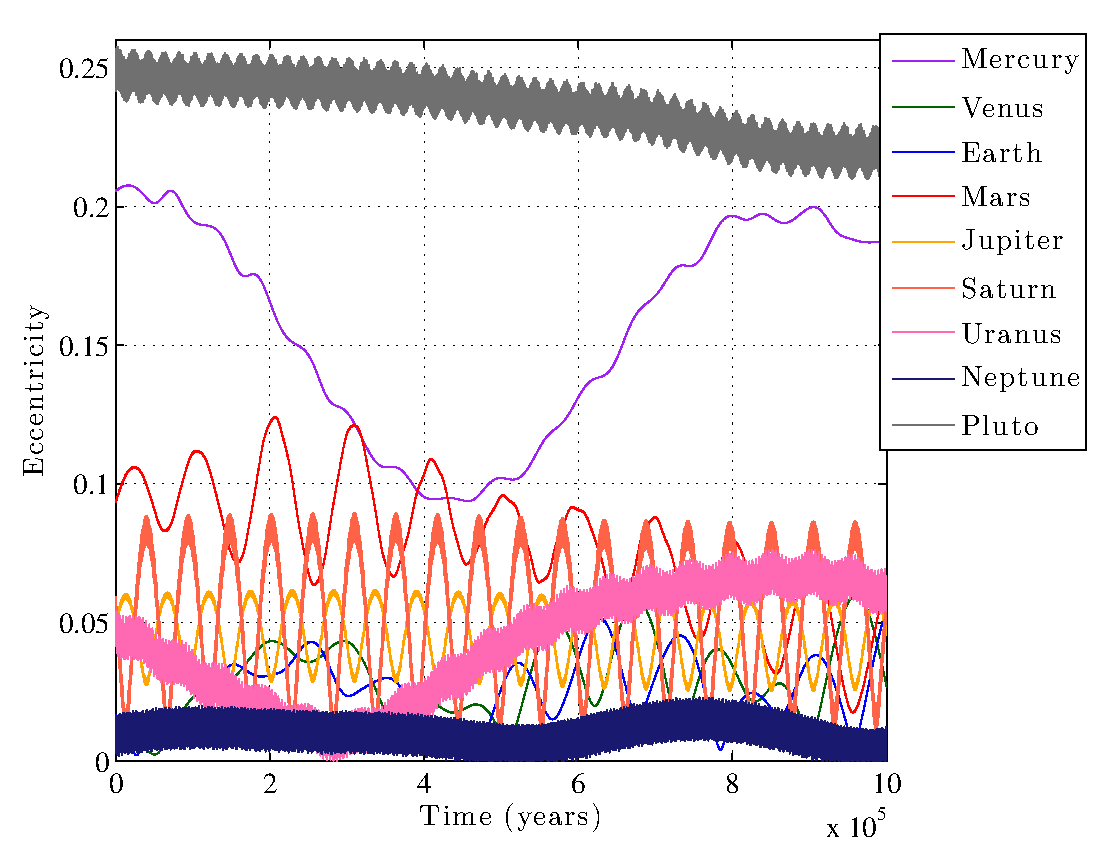
\includegraphics[width=6in]{./figures/eccenVar}
  \caption[Eccentricity variation]{ \label{fig:eccenVar} Variation in orbital eccentricities of solar system bodies over one million years.}
\end{figure}
In the case where there are only two bodies (say, a star and one planet), \refeq{eq:nbody} can be rewritten in terms of the separation vector between the pair, rather than with respect to some inertial origin:
\begin{equation}\label{eq:twoBody}
\fdddt{I}{\mf r_{P/S}} + (\mu_S + \mu_P) \frac{\mf r_{P/S}}{\Vert\mf r_{P/S}\Vert^3} = 0 \,,
\end{equation}
from which all of Kepler's laws and orbital equations can be derived.  Using Equations (\ref{eq:vec2orbelem1}) through (\ref{eq:vec2orbelemf}), we can see that in the multi-planet case, the Keplerian orbital elements represent instantaneous fits to \refeq{eq:twoBody}, which approximates the true system dynamics assuming that the combined effects due to all other bodies in the system are small compared to those due to the star.  Alternatively, we can find osculating Keplerian elements for multi-body systems that are time-varying, as in \reffig{fig:eccenVar}.
 
Of course, the Newtonian formulation is itself an approximation, with the true expressions for the motions of bodies in gravitational fields given by the Einstein field equations.  There are almost no cases in the modeling of planetary systems where it is necessary to use the field equations to calculate the exact metric tensor, but there may be observable general relativity effects in bodies orbiting closely to their parent stars (as happens, for example, with Mercury in our solar system \citep{fabrycky2010non}).  In these cases, it is possible to model some of the `post-Newtonian' effects by expanding the field equations to first order in the ratio of orbital velocity and the speed of light.  One example of this is the Einstein-Infeld-Hofmann equations of motion \citep{einstein1938gravitational,einstein1940gravitational}:
\begin{align}
\fdddt{I}{\mf r_{j/O}} = &\sum_{k\in Y} \frac{\mu_k(\mf r_{k/O} - \mf r_{j/O})}{\Vert \mf r_{k/O} - \mf r_{j/O}\Vert^3} 
+ \frac{1}{c^2}\sum_{k\in Y} \frac{\mu_k(\mf r_{k/O} - \mf r_{j/O})}{\Vert \mf r_{k/O} - \mf r_{j/O}\Vert^3}\left[  {}^I \mf v_{j/O} \cdot {}^I \mf v_{j/O} \phantom{\fdddt{I}{\mf r_{k/O}}}\right. \nonumber\\
&{} + 2 {}^I \mf v_{k/O} \cdot {}^I \mf v_{k/O} - 4 {}^I \mf v_{j/O} \cdot {}^I \mf v_{k/O} - \frac{3}{2}\left(\frac{(\mf r_{j/O} - \mf r_{k/O}) \cdot {}^I \mf v_{k/O} }{\Vert \mf r_{j/O} - \mf r_{k/O} \Vert}\right)^2 \nonumber\\
&\left. {} - 4\sum_{i \in Y} \frac{\mu_i}{\Vert \mf r_{j/O} - \mf r_{i/O}\Vert} - \sum_{i \in Z}\frac{\mu_i}{\Vert \mf r_{k/O} - \mf r_{i/O}\Vert} + \frac{1}{2}\left((\mf r_{k/O} - \mf r_{j/O})\cdot \fdddt{I}{\mf r_{k/O}}\right)\right] \nonumber \\
&{}+ \frac{1}{c^2}\sum_{k\in Y} \frac{\mu_k}{\Vert \mf r_{k/O} - \mf r_{j/O}\Vert^3}\left[ (\mf r_{j/O} -\mf r_{k/O} )\cdot (4 {}^I \mf v_{j/O} - 3  {}^I \mf v_{k/O} )\right] ( {}^I \mf v_{j/O}-  {}^I \mf v_{k/O} ) \nonumber \\
&{} + \frac{7}{2c^2} \sum_{k\in Y} \frac{\mu_k}{\Vert \mf r_{k/O} - \mf r_{j/O}\Vert}\fdddt{I}{\mf r_{k/O}}\,, \, j \in X \label{eq:einstein_nbody}
\end{align}
where  $c\addsymbol{$c$}{Speed of light}$ is the speed of light and $Z$ is the subset of $X$ not containing $k$:
\begin{equation}
Z \subset X : k \notin Z \,.
\end{equation}
Besides being functionally more complex than \refeq{eq:nbody}, this equation is also significantly more difficult to integrate as it contains velocity terms (invalidating a whole class of second-order integrators that are commonly used to integrate n-body systems) as well as acceleration terms, which require a fully implicit integrator.  Because of this, it is common practice to integrate only the Newtonian formulation, and to apply the post-Newtonian correction only when deviations due to general relativity effects become too pronounced to ignore\footnote{For further discussion on numerical integration see \S\ref{sec:gen_plan_sys}.}.

\section{The Point Spread Function}\label{sec:PSF}
Before proceeding to any discussion of specific detection methods, we need a standardized description of an imaging system, which will be used to develop the models for direct detection, doppler spectroscopy, and transit photometry (and is also applicable to some interferometers used for astrometry).  Following \citet{goodman2005introduction}, we assume the imaging system to act as a linear operator $\mc F$ such that,
\begin{equation}
\mc F: E_o(u,v) \rightarrow E_i(x,y)
\end{equation}
where $E_o(u,v)$ is the electric field transmitted by the object and $E_i(x,y)$ is the image electric field (with image coordinates $x,y$).  The input can be decomposed by taking advantage of the Dirac $\delta$ function as:
\begin{equation}
E_o(u,v) = \iint\limits_{-\infty}^{\quad \infty} E_o(\xi,\eta) \delta(u-\xi, v-\eta) \intd{\xi}\intd{\eta} \,,
\end{equation}
so that we can write:
\begin{equation}\label{eq:supInt}
E_i(x,y) = \iint\limits_{-\infty}^{\quad \infty} E_o(\xi,\eta) h(x,y,\xi,\eta) \intd{\xi}\intd{\eta} \,,
\end{equation}
where 
\begin{equation}
h(x,y,\xi,\eta)  = \mc F\left\{ \delta(u-\xi, v-\eta) \right\} \,.
\end{equation}
The superposition integral in \refeq{eq:supInt} can be used to characterize an imaging system by its response to unit impulses via the impulse response function $h$, known as the point spread function (PSF$\addsymbol{PSF}{Point spread function}$).  This function can be interpreted as the resulting image of an electric field emitted by a point source; any image can thus be built up from images of point sources distributed throughout the field of view.  With some assumptions, it can be shown that the function $\mc F$ is a Fourier transform, allowing us to express $h$ in terms of specific instrument properties \citep{hecht2002optics,bracewell2000fourier}.

Starting with an aperture $A$ in the $(u,v)$ plane, we form another plane $(x,y)$, a distance $z$ away.  By the Huygens-Fresnel principle,
\begin{equation}
E_z(x,y) = \frac{1}{i\lambda}  \iint\limits_{A(u,v)} E_o(u,v) e^{i\frac{2 \pi}{\lambda}\Vert \mf r \Vert} \frac{\cos\theta}{\Vert \mf r \Vert}  \intd{u}\intd{v}
\end{equation}
where $\lambda\addsymbol{$\lambda$}{Wavelength}$ is the wavelength, $\mf r$ is the vector between the point in $(x,y)$ and the point in $(u,v)$, and $\theta$ is the angle between $\mf r$ and the vector normal to the two planes, such that $\cos\theta = z/\Vert \mf r\Vert$.  This formulation is based on scalar diffraction theory and assumes that $\Vert \mf r\Vert \gg \lambda$, i.e., that the image is many wavelengths from the aperture.

Applying the binomial expansion to the magnitude of $\mf r$, we have:
\begin{align}
\Vert \mf r \Vert &= z\sqrt{1 + \left(\frac{x-u}{z}\right)^2 + \left(\frac{y-v}{z}\right)^2}\\
& = z + \frac{z}{2}\left(\frac{x-u}{z}\right)^2+ \frac{z}{2} \left(\frac{y-v}{z}\right)^2 + \cdots
\end{align}
so we make the approximation:
\begin{equation} \label{eq:fresnelint}
E_z(x,y) \approx \frac{e^{i\frac{2\pi}{\lambda}z}}{i\lambda z}  \iint\limits_{A(u,v)} E_o(u,v) e^{i\frac{\pi}{\lambda z}\left[ (x - u)^2 + (y - v)^2\right]} \intd{u}\intd{v} \,.
\end{equation}
This expression, known as the Fresnel integral, can be seen to be a convolution\footnote{Strictly, the integral should be written with limits from $-\infty$ to $\infty$, in which case it is understood that $E_o(u,v)$ is zero outside of $A(u,v)$.}  between $E_o(u,v)$ and the kernel:
\begin{equation}
h(x,y) = \frac{e^{i\frac{2\pi}{\lambda}z}}{i\lambda z}e^{i\frac{\pi}{\lambda z}\left(x^2 + y^2\right)} \,.
\end{equation}
Because this is a Gaussian Kernel, the Fourier conjugate of $E_z$ can be written as:
\begin{equation}\label{eq:fourierConj}
\hat{E}_z(\xi,\eta) = e^{i\frac{2\pi}{\lambda}z} \hat{E}_o(\xi,\eta)e^{-i\pi \lambda z\left(\xi^2 + \eta^2\right)} \,.
\end{equation}
Similarly, \refeq{eq:fresnelint} can be rewritten as:
\begin{equation}\label{eq:fresnelint2}
E_z(x,y) = \frac{e^{i\frac{2\pi}{\lambda}z}}{i\lambda z}e^{i\frac{\pi}{\lambda z}\left(x^2 + y^2\right)} \iint\limits_{-\infty}^{\quad \infty} E_o(u,v)e^{i\frac{\pi}{\lambda z}\left(u^2 + v^2\right)}  e^{-i\frac{2\pi}{\lambda z}\left(xu +yv\right)} \intd{u}\intd{v} \,,
\end{equation}
which is a scaled Fourier transform of $E_o(u,v)e^{i\frac{\pi}{\lambda z}\left(u^2 + v^2\right)}$.

Assuming that there is a lens at the aperture plane with focal length $f$, \refeq{eq:fresnelint} can be used to express the field at the focal plane as:
\begin{equation}\label{eq:lensFourierTrans}
E_f(x,y) = \frac{e^{i\frac{2\pi}{\lambda}f}}{i\lambda f}e^{i\frac{\pi}{\lambda z}\left(x^2 + y^2\right)} \hat{E}_A\left(\frac{x}{\lambda f}, \frac{y}{\lambda f}\right)
\end{equation}
for
\begin{equation}
E_o(u,v) = E_A(u,v)e^{i\frac{\pi}{\lambda f}\left(u^2 + v^2\right)} \,. 
\end{equation}
Now, if the free space propagation before the lens is equal to $f$, then Equations (\ref{eq:lensFourierTrans}) and (\ref{eq:fourierConj}) combine to produce:
\begin{equation}
E_i(x,y) = \frac{1}{i\lambda f}e^{i\frac{\pi}{\lambda f}\left( \frac{1}{f} - \frac{1}{f}\right)\left(x^2 + y^2\right)} \hat{E}_o\left(\frac{x}{\lambda f}, \frac{y}{\lambda f}\right) =  \frac{1}{i\lambda f} \hat{E}_o\left(\frac{x}{\lambda f}, \frac{y}{\lambda f}\right)
\end{equation}
so that the electric field at the focal plane is simply the Fourier transform of the incoming field.

Returning to \refeq{eq:supInt}, the impulse response function can now be written as:
\begin{equation}
h(x,y) = \frac{1}{\lambda f} \iint\limits_{-\infty}^{\quad \infty} A(u,v) e^{-i\frac{2\pi}{\lambda f}\left(xu +yv\right)} \intd{u}\intd{v} \,.
\end{equation}
Since the effect of a lens is to take the Fourier transform of the incoming field, the intensity distribution of the image is given by
\begin{equation}
I_i(x,y) = \vert \hat{E}_0\vert^2 \,,
\end{equation}
and so we can write
\begin{equation}
I_i(x,y) = \kappa \iint\limits_{-\infty}^{\quad \infty} \vert h(\xi - u, v-\eta) \vert^2 I_o(u,v) \intd{u}\intd{v} \,,
\end{equation}
for real constant $\kappa$.
We can thus define the intensity impulse response, $\vert h\vert^2$, or point spread function:
\begin{equation}\label{eq:PSFdef}
\PSF (x,y) = \frac{1}{\lambda^2 f^2} \left\vert\iint\limits_{-\infty}^{\quad \infty} A(u,v) e^{-i\frac{2\pi}{\lambda f}\left(xu +yv\right)} \intd{u}\intd{v} \right\vert^2 \,.
\end{equation}
\refeq{eq:PSFdef} provides us with a way of characterizing the effects of the optical system, and thereby the ability to disentangle these from the true signal being measured.

\bigskip
\bigskip

The descriptions of planetary orbits, physical parameters and imaging systems laid out in the previous two sections make it possible to rigorously define exactly how the different detection methods find and observe planets, using a unified syntax which will prove very important in subsequent chapters.  In the next chapter, we will introduce the four detection method studied in this thesis and, using the groundwork laid here, we will be able to describe what form the data from each detection method will take, and develop expressions for the observables and constraints of each method. 



 






